\documentclass[10pt,a4paper]{article}
\usepackage[margin=1.7cm]{geometry}
\usepackage{graphicx}
\usepackage{amsmath}
\usepackage{booktabs}
\usepackage{caption}
\usepackage[hidelinks]{hyperref}
\newcommand{\COtwo}{CO\textsubscript{2}\xspace}
\usepackage{xspace}

\captionsetup{font=small}
\setlength{\parskip}{0.3em}

\title{\vspace{-1.5cm}Is Economic Growth Decoupling from \COtwo{} Emissions?\\
\large A cross-country analysis of the Our World in Data \COtwo{} dataset, 2005--2022}
\author{Your Name (Student ID) \\ \small MAT2007 Introduction to Programming, Maastricht University}
\date{October 2026}

\begin{document}
\maketitle
\vspace{-0.8cm}

\section*{Introduction}
Limiting global warming requires deep cuts in \COtwo{} emissions, while most
countries still pursue economic growth. Whether the two goals are compatible
depends on \emph{decoupling}. When \COtwo{} emissions grow more slowly than GDP,
we have \emph{relative} decoupling. When emissions fall while GDP keeps growing,
we have \emph{absolute} decoupling~\cite{ipcc}. A common objection to apparent
decoupling in rich countries is that they have only moved polluting production
abroad. In this report we ask: \textbf{how many countries have achieved absolute
decoupling since 2005? How does this depend on a country's income level? And does
the result survive when emissions are counted by consumption rather than
production?}

\section*{Dataset}
We use the \COtwo{} and Greenhouse Gas Emissions dataset published by Our World
in Data (OWID)~\cite{owid}. It is a single CSV file of about 14\,MB with 79
columns and 50\,411 rows, one per country (or region) per year. We use these
columns:
\begin{itemize}\setlength\itemsep{0em}
  \item \texttt{gdp}: GDP in constant international dollars (Maddison Project), available up to 2022;
  \item \texttt{co2}: annual territorial (production-based) fossil \COtwo{} emissions in Mt;
  \item \texttt{consumption\_co2}: emissions adjusted for trade, i.e.\ attributed to the country where the goods are consumed;
  \item \texttt{population}, \texttt{country}, \texttt{iso\_code}, \texttt{year}.
\end{itemize}
We clean the data in three steps. First, we remove regional aggregates
(rows with no ISO code or with an \texttt{OWID\_} code). Second, we keep only
countries with complete GDP, \COtwo{} and population data for every year from
2005 to 2022. Third, we drop countries with fewer than one million inhabitants.
This leaves $N=153$ countries. Consumption-based data exist for 116 of them.

\section*{Method}
The analysis is implemented in Python (\texttt{pandas}, \texttt{scipy},
\texttt{matplotlib}). For each country we fit a log-linear trend
$\ln X(t) = a + b\,t$ by least squares, separately for $X = $ GDP, territorial
\COtwo{} and consumption \COtwo{}. The average annual growth rate is
$r = 100\,(e^{b}-1)\,\%$. Its uncertainty, propagated from the standard error
of the slope, is $\sigma_r = 100\,e^{b}\,\sigma_b$. Fitting a trend uses all 18
years of data, so it is less sensitive to one-off years such as 2020 than a
simple start-to-end comparison would be. Each country is then classified:
\begin{itemize}\setlength\itemsep{0em}
  \item \emph{absolute decoupling}: $r_{\rm GDP} > 0$ and \COtwo{} decreasing at 95\% confidence, i.e.\ $r_{\rm CO_2} + 1.96\,\sigma_{r} < 0$;
  \item \emph{relative decoupling}: $0 < r_{\rm GDP}$ and $r_{\rm CO_2} < r_{\rm GDP}$ (and not absolute);
  \item \emph{no decoupling}: $r_{\rm CO_2} \geq r_{\rm GDP} > 0$;
  \item \emph{GDP decline}: $r_{\rm GDP} \leq 0$. Decoupling is not defined here (e.g.\ Greece, Italy, Venezuela).
\end{itemize}
Countries are divided into four income groups using the quartiles of their GDP
per capita in 2005. For the fraction of countries $p = k/n$ in a class we
quote the binomial uncertainty $\sigma_p = \sqrt{p(1-p)/n}$.

\section*{Results and discussion}
Figure~\ref{fig:scatter} shows the GDP growth rate against the territorial
\COtwo{} growth rate for all 153 countries. Using territorial emissions, the
countries split as follows:
$(22.2 \pm 3.4)\%$ absolute decoupling (34 countries),
$(43.8 \pm 4.0)\%$ relative decoupling,
$(26.8 \pm 3.6)\%$ no decoupling, and $(7.2\pm2.1)\%$ GDP decline.
Absolute decoupling is concentrated in rich economies. For example, the United
Kingdom grew by $(1.11\pm0.16)\%$/yr while its emissions fell by
$(3.54\pm0.15)\%$/yr. For the United States the corresponding figures are
$(1.68\pm0.10)\%$/yr and $-(1.22\pm0.14)\%$/yr, and for Germany
$(1.58\pm0.12)\%$/yr and $-(1.53\pm0.19)\%$/yr. China
($r_{\rm GDP}=7.05\%$, $r_{\rm CO_2}=3.51\%$) and India (6.27\%, 5.05\%) show
only relative decoupling. The initial income level and the \COtwo{} growth rate
are strongly anti-correlated (Spearman $\rho = -0.69$, $p \approx 10^{-22}$).

\begin{figure}[h]
  \centering
  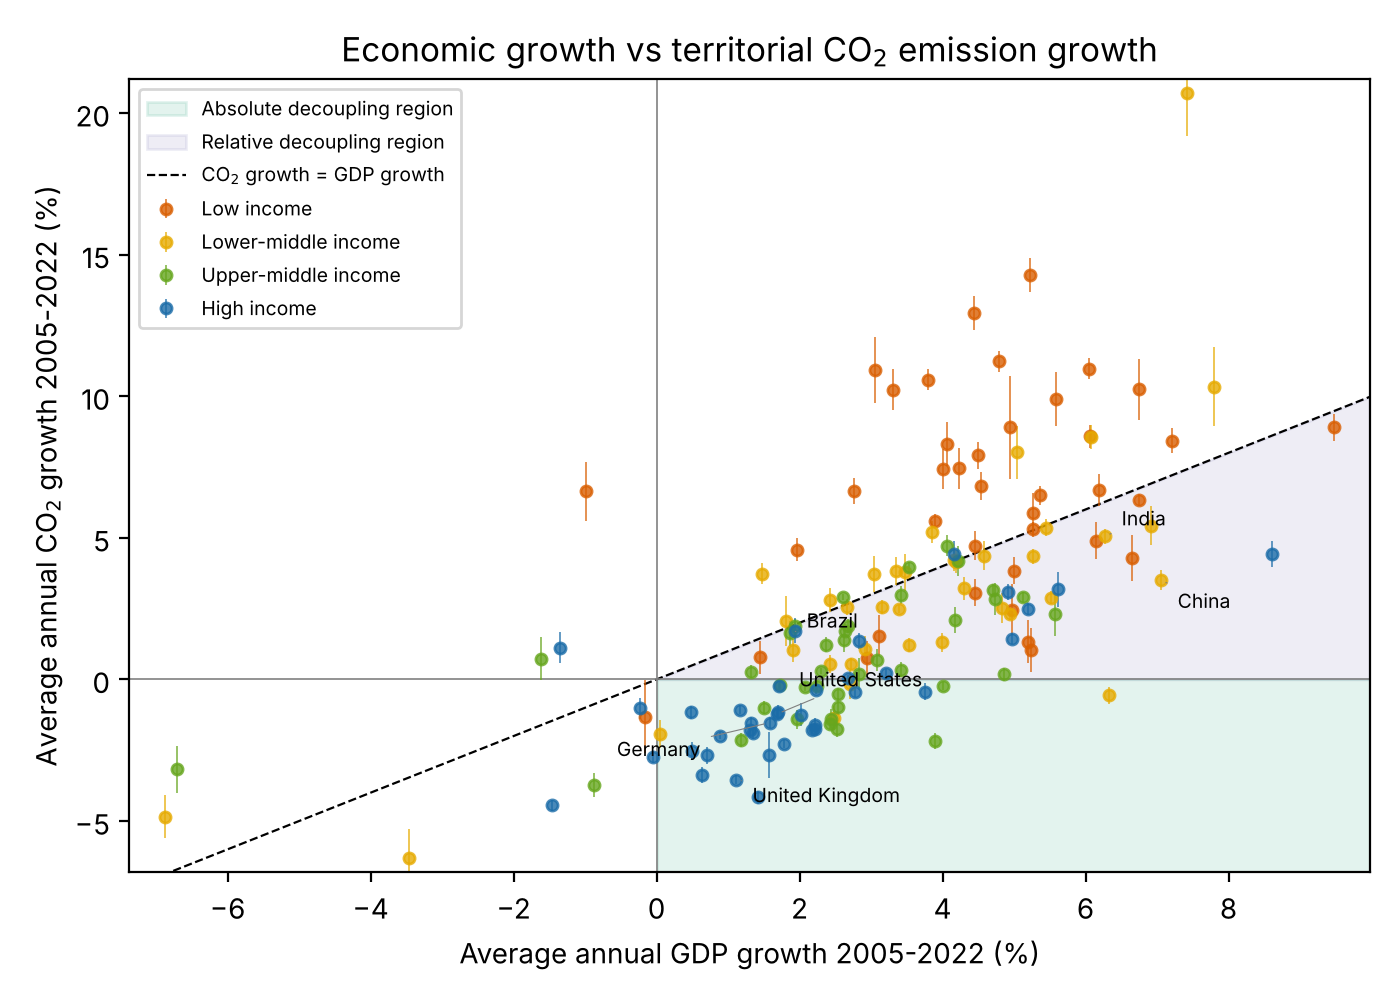
\includegraphics[width=0.56\linewidth]{../figures/growth_scatter.png}
  \vspace{-0.2cm}
  \caption{Average annual GDP growth versus territorial \COtwo{} growth,
  2005--2022. Each point is a country, coloured by income quartile in 2005. The error bars are the
  $1\sigma$ uncertainties of the fitted \COtwo{} trend. Points in the green region show
  absolute decoupling. Points in the purple region show relative decoupling.}
  \label{fig:scatter}
\end{figure}

\begin{figure}[h]
  \centering
  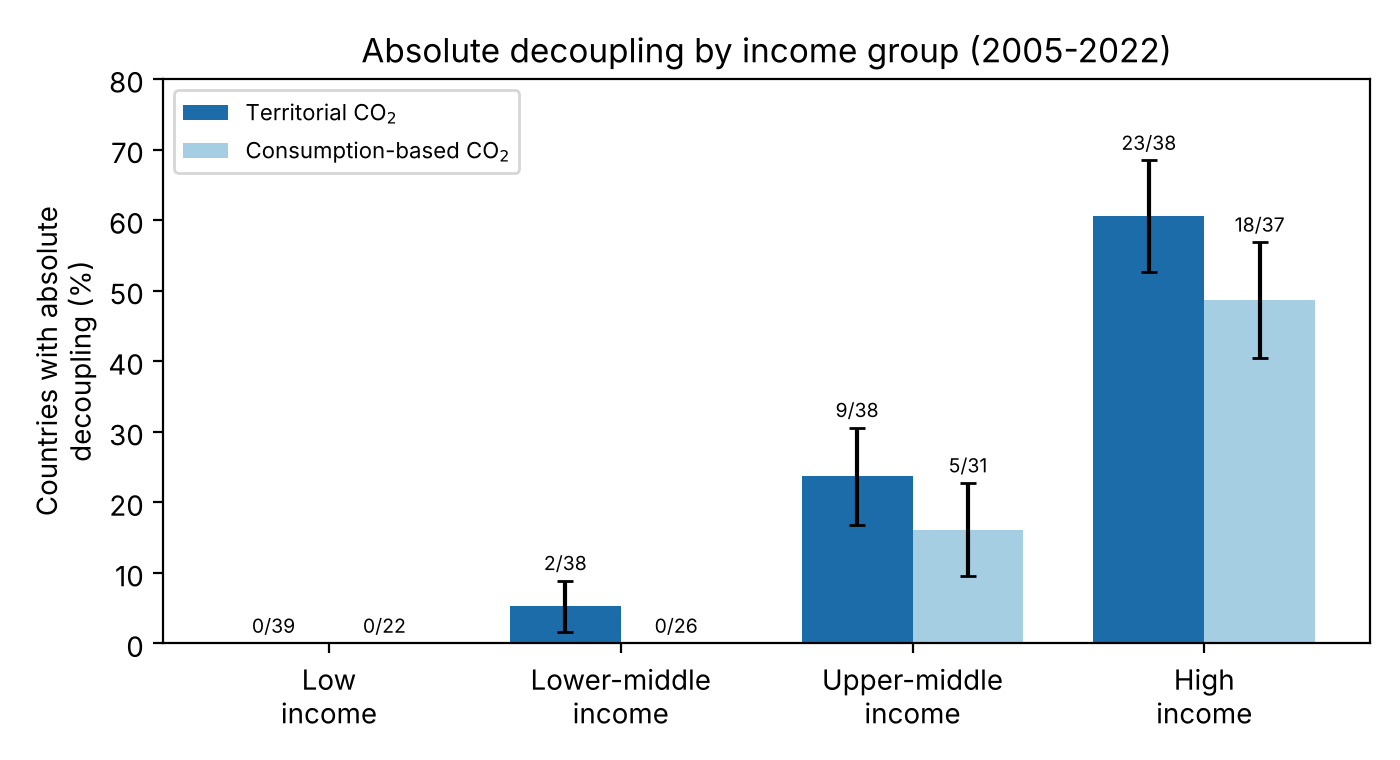
\includegraphics[width=0.54\linewidth]{../figures/decoupling_by_income.png}
  \vspace{-0.2cm}
  \caption{Fraction of countries with absolute decoupling in each income
  quartile, for territorial and consumption-based emissions. The error bars
  are binomial uncertainties. The labels above the bars give the raw counts $k/n$.}
  \label{fig:income}
\end{figure}

Figure~\ref{fig:income} quantifies the income dependence. No low-income
country (0/39) and only 2/38 lower-middle-income countries decoupled
absolutely, against $(60.5\pm7.9)\%$ (23/38) of high-income countries. The
difference between the high- and low-income groups is $0.61\pm0.08$, which is
$7.6\sigma$. Counting emissions by consumption lowers the high-income fraction
to $(48.6\pm8.2)\%$ (18/37), a reduction of $1.0\sigma$. Offshoring of
production therefore explains part of the apparent decoupling, but not most of
it. For example, the UK, the US, Germany and the Netherlands all still show
absolute decoupling on a consumption basis.

\textbf{Conclusion.} Absolute decoupling of GDP from \COtwo{} emissions is
real but limited. It occurred in about one country in five over 2005--2022,
almost exclusively in high- and upper-middle-income economies, and it largely
persists when trade is taken into account. However, even the decoupling
countries reduce emissions by only about 1--4\%/yr. This is well below the
roughly 6\%/yr global cut implied by 1.5\,$^\circ$C pathways (CO\textsubscript{2} about 48\% below 2019 levels by 2030)~\cite{ipcc}.
Most of the world, including the large emitters China and India, is still in
the relative-decoupling regime. One limitation is that the growth rates assume
a constant exponential trend, which ignores changes in trend within the period.

\vspace{-0.3cm}
\renewcommand{\refname}{\normalsize References}
\begin{thebibliography}{9}\setlength\itemsep{0em}\small
\bibitem{owid} Our World in Data, \emph{\COtwo{} and Greenhouse Gas Emissions dataset},
\url{https://github.com/owid/co2-data} (commit \texttt{382ee6c}, accessed October 2026).
\bibitem{ipcc} IPCC, \emph{Climate Change 2022: Mitigation of Climate Change}, Working Group III
contribution to the Sixth Assessment Report, Cambridge University Press (2022).
\end{thebibliography}

\end{document}
